\chapter{原理图}
\label{cha:china}
包括项目原理图和电路原理图

\section{项目原理图}
\begin{figure}[H] % use float package if you want it here
  \centering
  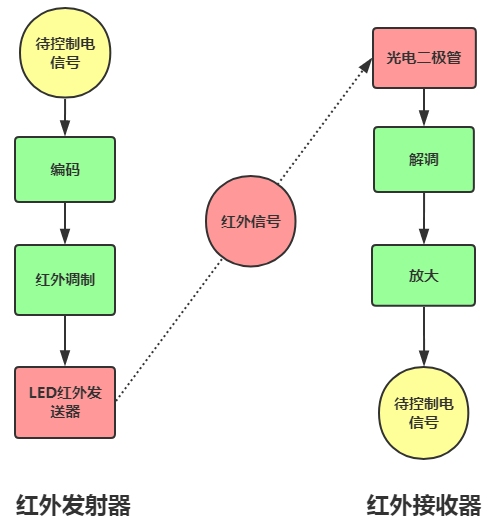
\includegraphics[width=0.7\textwidth]{2.png}
  \caption{项目原理图}
  \label{fig:xfig1}
\end{figure}
无线遥控器的原理就是发射机把控制的电信号\textbf{先编码,
然后再调制},红外调制或者无线调频、调幅,转换成无线信号发送出去。

接收机收到载有信息的无线电波\textbf{接收,放大,解码},得到原先的控制电信号,
把这个电信号再进行功率放大用来驱动相关的电气元件,实现无线的遥控。


\section{线路原理图}
\subsection{红外发射线路原理图}
\begin{figure}[H] % use float package if you want it here
  \centering
  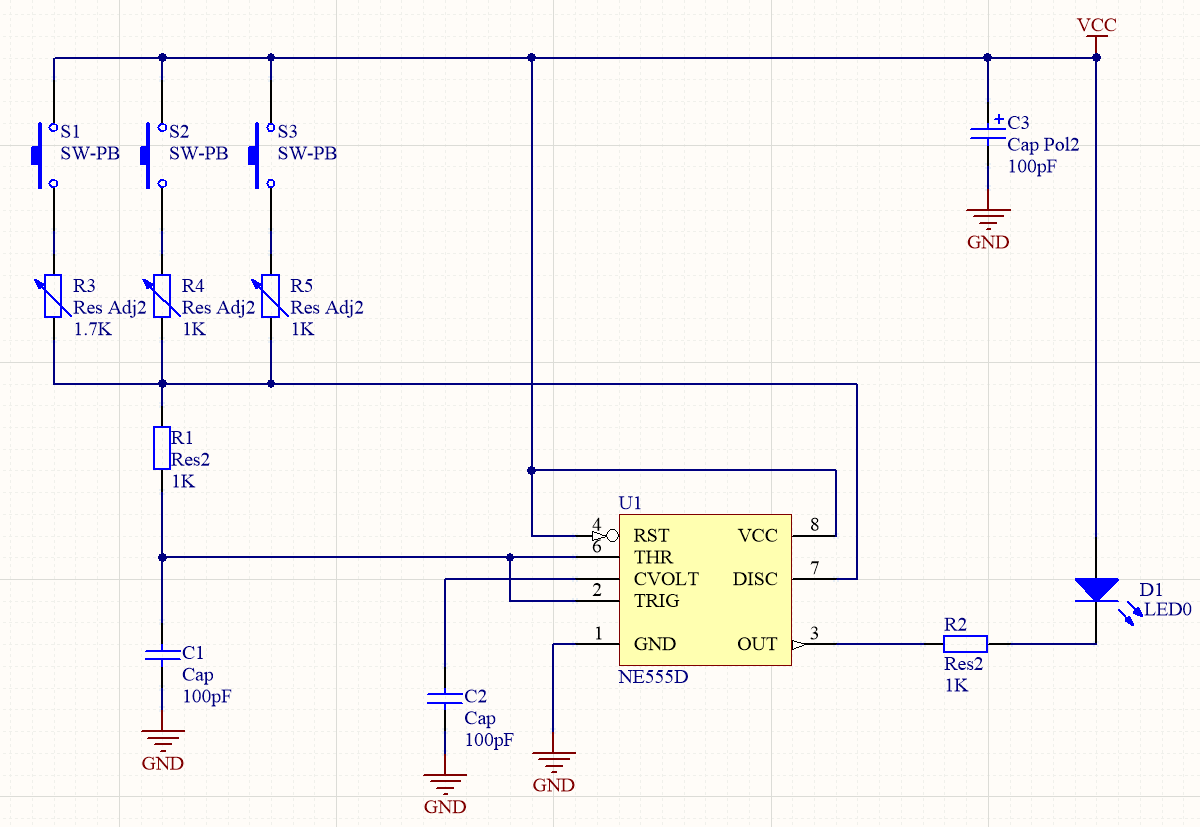
\includegraphics[width=1\textwidth]{3.png}
  \caption{红外发射线路原理图}
  \label{fig:xfig1}
\end{figure}
红外发射电路采用NE555接成振荡电路,如图所示。
振荡频率由SA1~SA3开关控制,改变开关位置,
即改变接入振荡电路的电阻RP1~RP3,调节RP1~RP3,
可以调节每一通道的具体频率。振荡脉冲由3号引脚输出,
驱动红外发光二极管发射红外光,即实现了用振荡脉冲对红外光的调制。

\subsection{红外接收线路原理图}
\begin{figure}[H] % use float package if you want it here
  \centering
  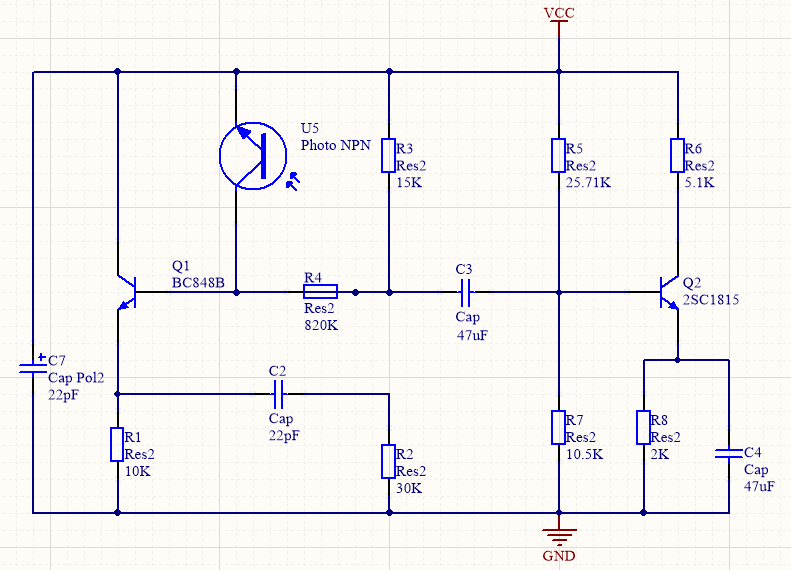
\includegraphics[width=1\textwidth]{3-2.png}
  \caption{红外接收线路原理图}
  \label{fig:xfig1}
\end{figure}
利用光电二极管接收上述红外发射电路发射的红外线,
利用光照强弱来改变电路中的电流,
通过BC848B和2SC1815三极管的放大和解调,输出得到期望的电压
